\documentclass[11pt,a4paper]{article}
\usepackage[margin=22mm]{geometry}
\usepackage[T1]{fontenc}
\usepackage{lmodern,graphicx,xcolor,microtype}
\usepackage[hidelinks]{hyperref}
\definecolor{teal}{HTML}{14655F}
\definecolor{ink}{HTML}{1C3036}
\pagestyle{empty}
\setlength{\parindent}{0pt}
\setlength{\parskip}{4pt}
\newcommand{\head}[2]{{\sffamily\bfseries\small\color{teal}SIGN LANGUAGE ALPHABET RECOGNITION\hfill RQ2\enspace / \enspace #1}\par
  \vspace{3pt}{\sffamily\bfseries\LARGE\color{ink}#2\par}
  \smallskip\textit{To what extent does applying a \(3\times3\) dilation filter recover visually plausible hand landmarks in ASL Alphabet training images for which MediaPipe initially detects no hand?}\par\smallskip}
\newcommand{\partof}[1]{\par\smallskip{\sffamily\bfseries\color{teal}#1}\par\nobreak}
\newcommand{\note}[1]{{\small\itshape #1}\par}
\newcommand{\photo}[3]{\begin{minipage}[t]{#1}\centering
  \includegraphics[width=\linewidth,height=34mm,keepaspectratio]{#2}\par{\small\sffamily #3}
  \end{minipage}}
\newcommand{\source}[2]{\href{#1}{\textit{#2}}}
\begin{document}
\head{01}{From one missed image to a dataset test}
\partof{Brief Introduction}
The alphabet classifier requires hand landmarks. N47 illustrates an earlier failure in the pipeline: a hand is visible, yet the original image yields no landmarks. RQ2 asks how often a second detection attempt can recover plausible landmarks among the other missed images.
\partof{Related Works}
MediaPipe Hand Landmarker returns estimated hand coordinates. Dilation changes the detector input by taking a local maximum in each colour channel. These two operations motivate a paired experiment in which the image changes while the detector is held fixed.
(\source{https://ai.google.dev/edge/mediapipe/solutions/vision/hand_landmarker}{MediaPipe};
\source{https://docs.opencv.org/3.4.20/db/df6/tutorial_erosion_dilatation.html}{OpenCV}.)
\partof{Methods and implementation}
First, process N47 in its original form and after one dilation with a square \(3\times3\) kernel. Use static-image mode and set the detection and presence thresholds to 0.50 in both runs. If the second run returns one valid hand, retain the settings for the A--Z study. Overlay the estimated points on the original pixels to inspect their placement.
\partof{Dataset and observed pilot result}
The baseline identified 17,598 training images with zero detected hands. N47 was selected because its failure was already known. In the pilot, its status changed from \texttt{no\_hand} to \texttt{ok} after dilation.

\begin{center}
\photo{.28\linewidth}{N47_original}{Original N47}\hfill
\photo{.28\linewidth}{N47_dilated}{Dilated input}\hfill
\photo{.36\linewidth}{N47_overlay}{Recovered points on original}
\end{center}
\note{Figure 1. Only the middle image is supplied to the detector on the second attempt. The dots in the right panel are its output.}
\partof{Results and discussion for the main study}
Set aside N47 and all previously inspected pilot images. Report the number with visually plausible recovery out of all remaining eligible misses. The N47 comparison establishes feasibility for one image. The dataset experiment determines the frequency of this outcome.

\newpage
\head{02}{Measuring how much training data can be recovered}
\partof{Brief Introduction}
Landmark extraction determines which images can enter the alphabet classifier. RQ2 quantifies how many initially missed images could become eligible if dilation were used as a second attempt.
\partof{Related Works}
When reviewing preprocessing studies, distinguish detection coverage from classification accuracy. A result calculated only on successfully detected hands cannot establish how many previously missed images a filter recovers. Use this distinction to select and discuss the empirical studies found in Google Scholar.
\partof{Dataset}
The original A--Z training folders contain 3,000 photos per letter. The baseline outcomes below define the population for RQ2. Only the zero-hand group enters the recovery experiment.

\begin{center}
\begin{tabular}{lr}
\hline
\textsf{Baseline outcome} & \textsf{Training images}\\\hline
One valid hand & 60,251\\
Multiple hands & 151\\
\textbf{Zero hands} & \textbf{17,598}\\\hline
Total & 78,000\\\hline
\end{tabular}
\end{center}
\note{Table 1. Original A--Z training inventory before image preprocessing.}
\partof{Methods and implementation}
Use N47 to verify the second-attempt procedure. Exclude development examples with known outcomes and record the remaining count. Apply the same \(3\times3\) dilation once to each remaining baseline miss, keeping model and thresholds fixed. Link both outcomes by original image ID. Inspect the landmarks from every technically successful recovery using a prespecified visual rubric.
\partof{Results}
In the exploratory, letter-balanced pilot, 130 of 520 initially missed images (25.0\%) yielded one valid detection after dilation. This measures technical recovery. For the main study, report two fractions with the same denominator: images yielding one valid detection divided by eligible misses, and visually plausible recoveries divided by eligible misses.
\partof{Discussion}
Each letter contributed 20 misses to the pilot, although letters contribute different numbers of misses to the dataset. Multiplying 25.0\% by 17,598 would therefore give an unjustified estimate. Report the observed total from the remaining images, with per-letter counts if space permits.

\newpage
\head{03}{Checking whether recovered points follow the hand}
\partof{Brief Introduction}
A second detection can produce a set of coordinates even when some points are difficult to reconcile with the visible fingers. RQ2 therefore includes a visual assessment before a recovered image is counted as a candidate for training.
\partof{Related Works}
MediaPipe estimates a hand configuration from image data. The distinction between an estimated and a visible joint matters for signs with overlapping fingers. For this study, the original photograph serves as a reference for the visible anatomy. (\source{https://ai.google.dev/edge/mediapipe/solutions/vision/hand_landmarker}{MediaPipe Hand Landmarker}.)
\partof{Dataset and methods}
Use N47 as a worked example to define the review procedure. Freeze that procedure before examining the remaining A--Z zero-hand photos, excluding previously inspected pilot examples. Run the filter once per photo with the same square kernel and detector thresholds. For each recovered hand, place the estimated points on the original photo at matching coordinates.

\begin{center}
\begin{minipage}{.30\linewidth}\centering
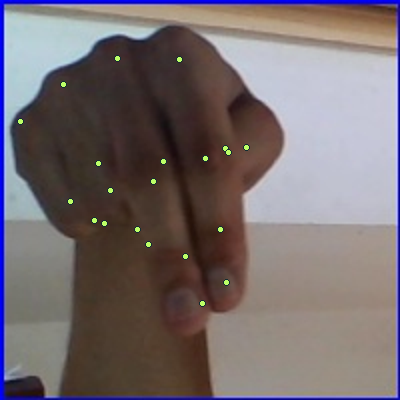
\includegraphics[width=35mm]{N47_overlay}
\end{minipage}\hfill
\begin{minipage}{.63\linewidth}\small
\textsf{\bfseries Visual review of N47}\\[3pt]
Is the wrist point at the wrist? Do the points follow the visible fingers? Where the fingers overlap, is there enough visual evidence to judge their placement?
\end{minipage}
\end{center}
\note{Figure 1. The overlay illustrates the review task. A visual judgement for N47 is deliberately left to the reviewer.}
\partof{Implementation and results}
Give each technically recovered image one review label. Use \emph{plausible} when the wrist and visible finger paths align with the hand, \emph{implausible} for a clear anatomical mismatch, and \emph{uncertain} when occlusion prevents a judgement. Record a brief reason. Report all three counts and the number without technical recovery. The primary outcome is the plausible count divided by all eligible misses.
\partof{Discussion}
This estimate describes the proportion of missed images that pass the specified visual screen. A second reviewer can independently assess a prespecified subset to examine consistency. Without annotated joint locations, visual agreement supports a plausibility judgement but does not quantify coordinate error. The effect on letter classification requires a separate evaluation.
\end{document}
